\chapter{Molecular modeling of biological membranes}
\label{chap:methods}

Biological membranes are of a great interest in biology and biophysics. 
The tools and methods that enable their research have greatly evolved over the last decades. 
Nowadays, there is a plethora of membrane models and experimental methods, 
each having its benefits and drawbacks \citep{REF} \todoi{1-2 chosen reviews, everything else in prev chapter}
(see section~\ref{sec:modelmemb} in chapter~\ref{chap:intro} for a detailed overview). 

Molecular simulation can be considered as one of the newer approaches in this field. 
Starting with simple membrane models \citep{REF} \todoi{REF: few old/new simulation works},
simulation of membranes has evolved into a field of computational biophysics
that is capable of answering fundamental questions.
The recent progress in computational resources and algorithms
has allowed the simulations to grow in spatial scales and composition complexity
bringing more relevance for applications in biology. \citep{REF: CECAM workshop} \todoi{REF to CECAM workshop 2018 Lugano}

Molecular dynamics simulations of biological membranes employ classical particle-based models of molecules. 
Vast majority of the models are built using classical non-polarizable particles, 
each representing an individual atom (atomistic models), 
or a group of atoms (united-atom or coarse grained models). 
The following classical models belong among the most succesful:
\begin{itemize}
 \item Atomistic
 \begin{itemize}
   \item CHARMM \citep{klauda10}
   \item Slipids \citep{jambeck12, jambeck12b}
   \item OPLS lipids by \citet{maciejewski14}
   \item Lipid14 \citep{dickson14}
  \end{itemize}

 \item Coarse grained
 \begin{itemize}
   \item MARTINI \citep{marrink07}
   \item Berger \citep{Berger97}
   \item CHARMM-UA \citep{lee14}
  \end{itemize}
\end{itemize}

Despite all successes and valuable insights simulations have provided, 
there is still a large room for possible improvements of the current simulation models. 
For example, recent studies by \citet{botan15, catte16} has shown 
that both structure and interaction of phospholipid models require further optimization 
in order to become capable of interpreting solid state NMR experiments. 
In particular, we have discovered that 
the lack of polarizability is a major issue in any of the models 
from the above mentioned works \citep{botan15, catte16}
when interactions with charged moieties become important. 
Several possible ways for embedding polarizability into simulations, both explicit and implicit, 
will be introduced in the following sections. 





\section{Classical molecular dynamics simulations}

Classical molecular dynamics simulation is used to provide insight into the dynamics and structure of the particles. 
\todo{Following taken from my diploma thesis directly -- to be modified!}
% Intro, Usage, boundaries (volume, time)
  Molecular dynamics simulations (MD) represent a branch of computational methodologies that can be desribed as theoretical experiments. 
  Their usage lays usually in desctiption of equilibrium states or in an assassement of evolution of non-equilibrium states.
  By running a computer simulation with subsequent application of statistical analysis, distributions of physical properties are usually obtained. 
  These methods were tradationally used in conjunction with experiments to help their interpretation and to test the theories behind both studies. After many years of development, molecular simulations are even used for prediction nowadays.

% I challenge you to a duel through time and space. 
  There are apparent advantages over experiments. Simulations can be used in cases when the experiment would be hard to accomplish; the resolution in time and space is easily reached. An evident disadvantage is, however, that the performed simulation is always only a theoretical model of a reality. 

 % Few words about propagators and how they should behave

In classical MD simulations, though, Newton equations of motion are used instead since the studied system are represented classicaly -- atoms are embodied by point masses with point partial charges; the exerting forces are defined by an approximate interaction potential (see section \ref{inter-pot}). 


   Interaction of atoms was generally described in the previous sections using an interaction potential $V$. Force fields represent one of its types.

     Force field is an empirical potential. It can be obtained by fitting a particular mathematical formula to an experiment or ab-initio calculations. It is the fastest method yet the most inaccurate. Chemistry can be made only in very special forms of it (for example EVB, empirical valence bond). It allows us to study large systems conatining tens or even hunderds of thousands atoms. More information will be given in the following sections.


  Classical force fields are pairwise additive. Amber, Charmm, OPLS, UFF and many others belong to this group. 

  Amber may serve as an example of a simple classical force field potential form:
 % Amber potential energy form:
\begin{eqnarray}  \label{amber}
  V = & \displaystyle \sum _{bonds} K_b (r-r_{eq})^2 + \sum _{angles} K_\Theta (\Theta-\Theta_{eq})^2 + \\ \nonumber
      & \displaystyle \sum _{dihedrals} \frac{1}{2} V_n (1+\cos(n\phi -\delta)) + \sum _{i<j} \left [ s_{ij} ^{VdW} \left( \frac{A_{ij}}{r_{ij} ^{12}} - \frac{B_{ij}}{r_{ij} ^6} \right ) + s_{ij}^q \frac{q_i q_j}{\epsilon \, r_{ij}} \right ]
\end{eqnarray}
  Non-bonded interaction are usually evaluated only for atoms separated by more than 3 bonds, as the interactions are already included in the bond stretching and angle bendig terms. 
  The number of non-bonded terms scales approximately quadratically with the size of the system and so it takes the most of the time of evaluation of the interaction potential.

   The core of a force field is the  definition of the potential. The mathematical form varies among different types of force fields; the harmonic potential is the most common, though, as it usually describes the potential in equilibrius position well. By fitting the formula to an experimental or ab-inition data, parameters are obtained for the various terms. Force fields for smaller systems (for example salts dissolved in water) can more precise than for larger systems, where the formula must be more general due to the high number of types of interactions. 

 When describing a molecule it's most often an advantage to use the internal coordinates. Instead of using the coupled $3N$ cartesian coordinates, the internal coordinates allow us to use the local symmetry of a molecule, which simplifies the formula. 
 These terms appear in force fields for biophysical applications most frequently: 
 bond stretching, angle bending, dihedral torsions.


  Except the bonding terms that describe the interactions of molecules separated by less than four bonds there also must be such terms that incorporate the strong electrostatic interaction and dispersion. 

  Electrostatic interaction has a long range impact meaning that its contributions from an infinite distance don't vanish and can't be neglected. A multipole expansion is used for its description: the 1\textsuperscript{st} term is a monopole (charged molecules, ions); 2\textsuperscript{ns} is a dipole that is usually present in all structures (for ex. water); 3\textsuperscript{rd} is a quadrupole etc.

  Charges on atoms are represented in that manner. The most important part plays the monopole. For that reason atoms are simplified as partial point charges. If a better precision is needed, dipoles can be added, though it's not a common case to do so. The dipole moment can be added by either specifying a dipole or by adding point charges representing it. The latter method can lead to different results due to the ambiguous determination of the representing charges. 

  As the electrostatic interaction is among the strongest even in neutral systems, its precise treatment is eminent. Ways how to deal with its long ranged nature follow in subsequent sections. 



  Ewald summation: When periodic boundary conditions for bulk compensation are used, the long range contribution to the electrostatic interaction cannot be neglected. If the system is neutral, it can be treated in a more efficient manner if the summation over distant charges is done in Fourier space rather than in real space. In a case of a charged system, the summation would not converge. 

  The procedure is that the contributions are divided into two groups depending on their distance from the center. The nearer charges are summed in real space. The further charges are formally treated as delta functions, and a gaussian curve with approximately the same but opposite charge is added to each of them. With such tuning the sum in real space becomes convergent. To compensate the added gaussians, their inversion is summed in the reciprocal Fourier space, where it converges better than in real space. 
% aplikace v programech -- fast FT, P$^3$M (par-par-particle mesh), PME, SPME (smooth PME)



  Van der Waals: When two atoms draw nearer their electronic structure changes due to electrostatic interaction and electronic correlation. As a consequence, even neutral atoms may attract each other by induced dipoles. The tendency to form them is specified by polarizability, which is a quantity that decribes the tendency of atoms to polarize themselves in an outer electric field. 

  Besides polarizibility, that was briefly introduced in previous sections, there is also a dispersion interaction that describes electronic correlation. Introduction of such forces is crucial with the point charge approximation as oppositely charged atoms would collapse into each other otherwise.

  The force is not strong; it's attractive in a distance $r$ from the source and is approximately proportional to $\frac{1}{r^6}$. The dispersion force is repulsive when atoms are near and the electronic orbital overlap a lot. This is approximately proportional to $ e^{-\alpha r} $.


  Lennard-Jones form doesn't suffer from this artefact. Accordingly to its form it is commonly reffered to as (12,6) potential:
\begin{equation}
   U_{VdW-LJ} =  \frac{A_{ij}}{r_{ij}^{12}} - \frac{B_{ij}}{r_{ij}^6} = \epsilon _{ij} \left [ \left (\frac{\sigma _{ij}}{r_{ij}} \right )^{12} - 2 \left ( \frac{\sigma _{ij}}{r_{ij}} \right )^6 \right ]
\end{equation}
  where $\epsilon$ denotes the depth of the minimum and $\sigma$ is the equilibrius position. 

  It's unusual to define parameters for every pair of atomic types in a force field. The specified parameters often refer to the interaction of two atoms of the same type. The rest of the parateres are obtained via mixing rules, which definition differs among forcefields. The most common mixing rules are Lorentz-Berthelot's:
\begin{equation}
 \sigma _{ij} = \frac{1}{2} (\sigma _{ii} + \sigma _{jj}) \, ; \quad \epsilon _{ij} = \sqrt{\epsilon _{ii} \, \epsilon _{jj}} 
\end{equation}
%\poznmini{souvisí s optikou -- index lomu }









\section{Including polarizability}

  Lit. research (history) on how people include polarizability in classical simulations. 

\subsection{Explicit treatment of electronic polarizability}

 Joint subsection on Drude particles and polarizable dipoles, the most common ways of introducing polarizability explicitly into the MD simulation. 

\subsection{Electronic continuum correction as implicit treatment of electronic polarizability}

The lack of electronic polarizability in standard MD force fields has been considered a serious issue since the early days of lipid bilayer simulations. In this work, we circumvent the demanding explicit inclusion of electronic polarization effects~\citep{lucas12, chowdhary13} by accounting for the electronic part of polarizability in lipid bilayer simulations implicitly via the electronic continuum correction (ECC)~\citep{leontyev11}. Technically, this is similar to the phenomenological charge-scaling applied in earlier studies of surfactants, lipids or ionic liquids \citep{jonsson86, egberts94, beichel14}. However, the present concept of ECC is physically well justified and has theoretical support~\citep{leontyev09, leontyev10, leontyev11, leontyev14}. 
 
According to ECC, the electronic polarizability can be included into non-polarizable MD in a mean-field way by  
embedding the ions in a homogeneous dielectric continuum with a dielectric constant $\epsilon_{el}$, which is the electronic part of the dielectric constant of the medium~\citep{leontyev11}. Following Coulomb's law,  ECC can be directly incorporated by scaling the charges with a constant scaling factor of $f_q = \epsilon _{el} ^{-1/2}$, yielding 
\begin{equation} 
Q^{ECC} = f_q \cdot Q 
\end{equation} 
for the ECC corrected charges.  
Given that the  high frequency dielectric constant of water is $\epsilon _{el} = 1.78$ (\textit{i.e.,} the square of the refraction index), the scaling factor for ions in water is roughly $f_q \approx 0.75$. This scaling factor significantly improves the accuracy of simulations of solvated ions, when quantitatively compared with neutron scattering data \citep{kohagen14,kohagen16, Pluharova2014, martinek17}. 
It is important to note that the value of the 
high frequency dielectric constant  
is around 2 for almost any biologically relevant environment \citep{leontyev11}. 
The dielectric discontinuity in a lipid bilayer thus arises only 
from the orientational polarization of the molecules, which is accounted for explicitly in standard MD simulations.  
Therefore, the same correction for the electronic polarizability can be  
applied throughout the lipid bilayer/aqueous solution interface. 
 
While using the scaling factor of $f_q = 0.75$ for ions in water is well justified in the ECC theory \citep{leontyev11}, it is not clear whether the same factor should be applied to partial charges used to describe molecules in MD models, e.g., lipids in our case \citep{leontyev14}. Unlike the total charge of an ion, atomic partial charges within molecules are not physical observables. Several computational schemes exist for the assignment of partial charges for biomolecules~\citep{Hu2007}, with the restrained electrostatic potential method (RESP) being commonly used~\citep{RESP_paper, Singh1984}. Considering that water is often included in RESP calculations or charges are refined to improve certain experimental observables, the electronic polarizability effects of the solvent may to some extent be included in standard force fields~\citep{RESP_paper, Singh1984, jorgensen96, ipolq2013, benavides17}. Thus, our application of the scaling factor, $f_q$, to existing partial charges in molecules does not necessarily follow $f_q = \epsilon _{el} ^{-1/2}$. Instead, a consistent scaling factor should lie between the value of 0.75  (\textit{i.e.,} no electronic polarizability included in the original partial charges) and 1 (\textit{i.e.,} electronic polarizability fully included in the original partial charges).  
 



\section{Implicitly polarizable classical MD models of lipids using ECC}

\textbf{ Change the following text and include PE and PS into this seciton. 
         Define ECC-lipids. Introduce all lipids in this section. }

Here we develop a ECC-POPC lipid model that accurately describes binding  
of sodium and calcium ions to the POPC  lipid bilayer.  
The Lipid14~\citep{dickson14} force field  
(available in a Gromacs format from Ref. \citep{lipid14files}) was used as a starting  
point since  
it provides the most accurate response of the head groups to ions among the available  
lipid models (see Figs.~2~and~5 in Ref.~\citep{catte16}). Additionally, the Lipid14 model  
provides relatively realistic head group, glycerol backbone, and acyl chain structures~\citep{dickson14,botan15}. 
We applied the ECC correction  
to the Lipid14 model of POPC by scaling  
partial charges of the head group, glycerol  
backbone, and carbonyl regions.  
These are the polar parts of phospholipids which can  
contribute to the cation binding.  
 
To reproduce the experimental ion binding affinities, 
we scanned possible values of the scaling factor from the interval $f_q~\in~(0.75, 1.0)$. 
The ion binding affinity was benchmarked against experiments 
using the head group order parameters and the electrometer concept \citep{seelig87,catte16}, 
as discussed more detail in the next section. 
Scaling down the partial charges reduced the ion binding affinity. 
We found the most accurate ion binding affinities with a scaling factor of $f_q = 0.8$, 
which is only slightly higher than the ECC one ($f_q=0.75$). 
Note that common empirical scaling factors for monovalent ions in water are 0.8 or
even closer to unity \citep{benavides17,skinner14,nacleps}.  In contrast, modern force fields
for ionic liquids suggest values of 0.6--0.65, which are lower than $\epsilon^{-1/2}_{el}$\citep{holm14}.
Directly applying 
the 0.8 scaling to the partial charges of the head group, the glycerol backbone, and 
the carbonyls reduced the area per lipid to 60~Å$^2$. This area is smaller than in the 
original Lipid14 model ($65.6 \pm 0.5$~Å$^2$)~\citep{dickson14} and in experiments 
(64.3~Å$^2$) \citep{kucerka11}. The decrease of the area per lipid arises from a 
reduced hydration of the lipid head group region after scaling of the partial charges, which effectively 
reduces the head group polarity. We solve this problem by slightly reducing the effective radii of 
the modified head group atoms via lowering the $\sigma$ parameters in the Lennard-Jones potential by a 
factor of $f_\sigma = 0.89$. The same approach was successfully adopted for the ECC ions in aqueous 
solutions previously \citep{kohagen14, kohagen16, Pluharova2014, martinek17}. After reducing the head group atoms $\sigma$ parameters, the area per molecule is restored to the experimental value (Table~\ref{tab:apls}).  


\subsection{Structural parameters of model membranes with ECC-lipids: Agreement with experiments} 
 
%%%%%%%%%%%%%%%%%%%%%%%%%%%%%%%%%%%%%%%%%%%%%%%%%%%%%%%%%%%%%%
% problem solved: NO line breaks in the caption!
\begin{figure}[tb!] 
  \centering 
  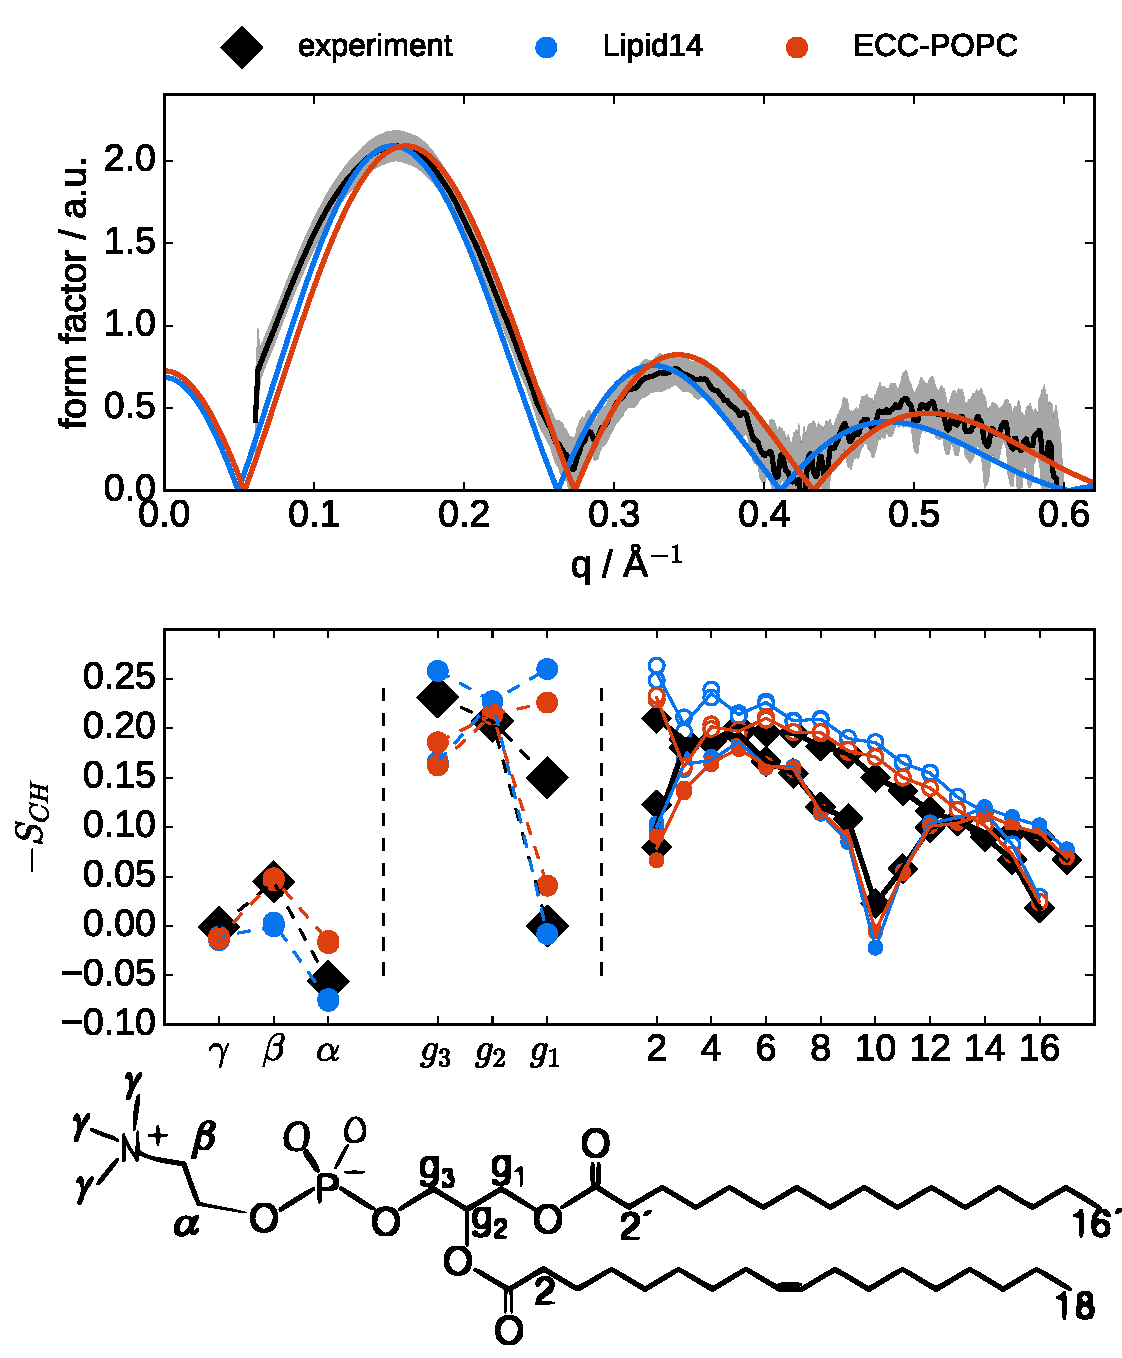
\includegraphics[width=8.2cm]{../img/ecc_popc/Order-parameters_form-factors_exp-L14-ECCL17_q80_sig89_POPC-struct.pdf} 
  \caption{ \label{simVSexpNOions} 
    Top: X-ray scattering form factors from simulations with the Lipid14 \citep{dickson14} and 
    the ECC-POPC models compared with experiments~\citep{kucerka11} at 303~K. 
    Middle: Order parameters of POPC head group, glycerol backbone and acyl chains  
    from simulations with the Lipid14 \citep{dickson14} and the ECC-POPC models 
    compared with experiments \citep{ferreira13} at 300~K. 
    The size of the markers for the head group order parameters correspond to 
    the error estimate $\pm 0.02$ for experiments \citep{botan15,ollila16}, 
    while the error estimate for simulations is $\pm 0.005$
    (Bayesian estimate of 95\% confidence interval \citep{scipy}).
    The size of the points for acyl chains are decreased by a factor of 3 to improve the clarity of the plot.
    Open/closed symbols are used for palmitoyl/oleoyl chains of POPC. 
    Bottom: The chemical structure of POPC and the labeling of the carbon segments. 
  }  
\end{figure} 


\begin{figure}[tb!] 
  \centering 
  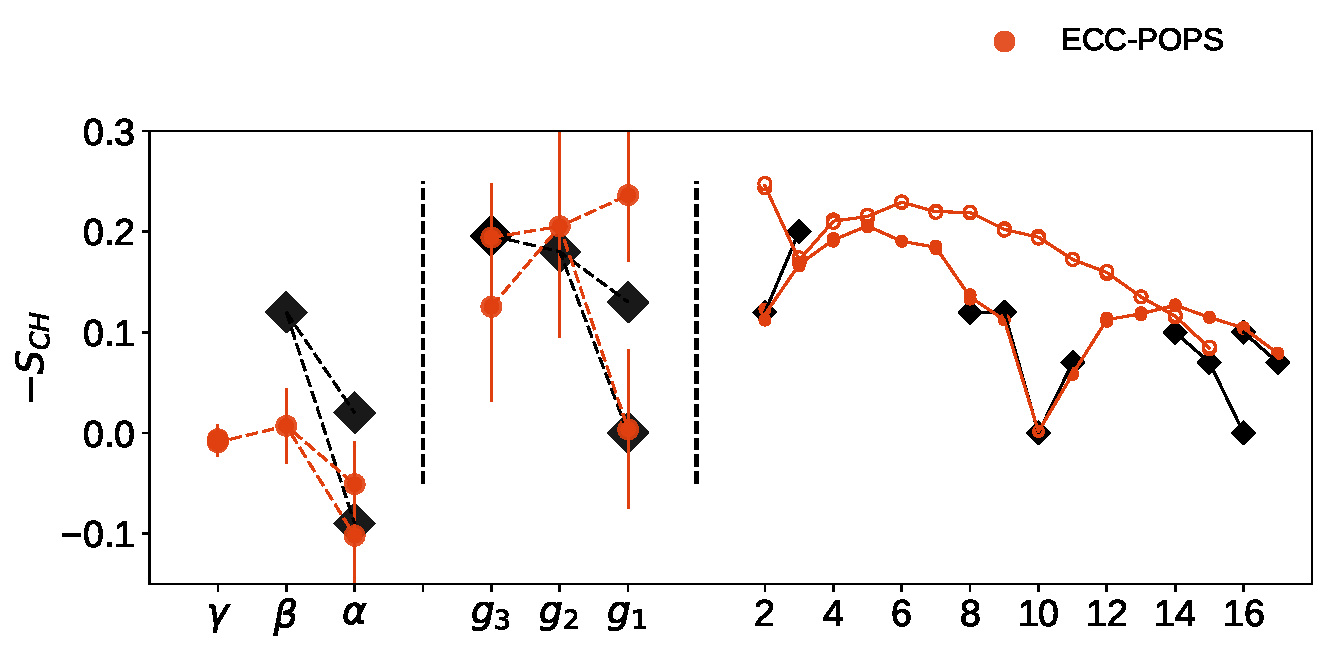
\includegraphics[width=\figwidth]{../img/ecc_pops/order_parameters_actual_pure-POPS.pdf} 
  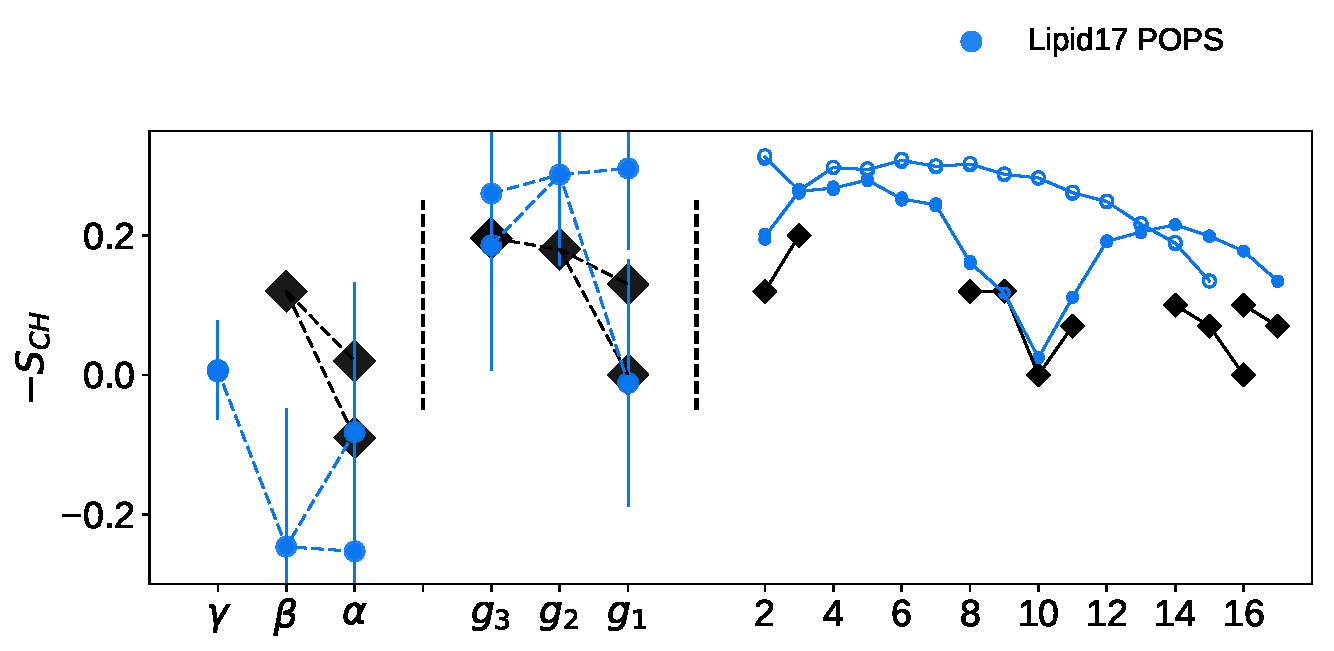
\includegraphics[width=\figwidth]{../img/ecc_pops/l17/order_parameters_actual_pure-POPS.pdf} 
  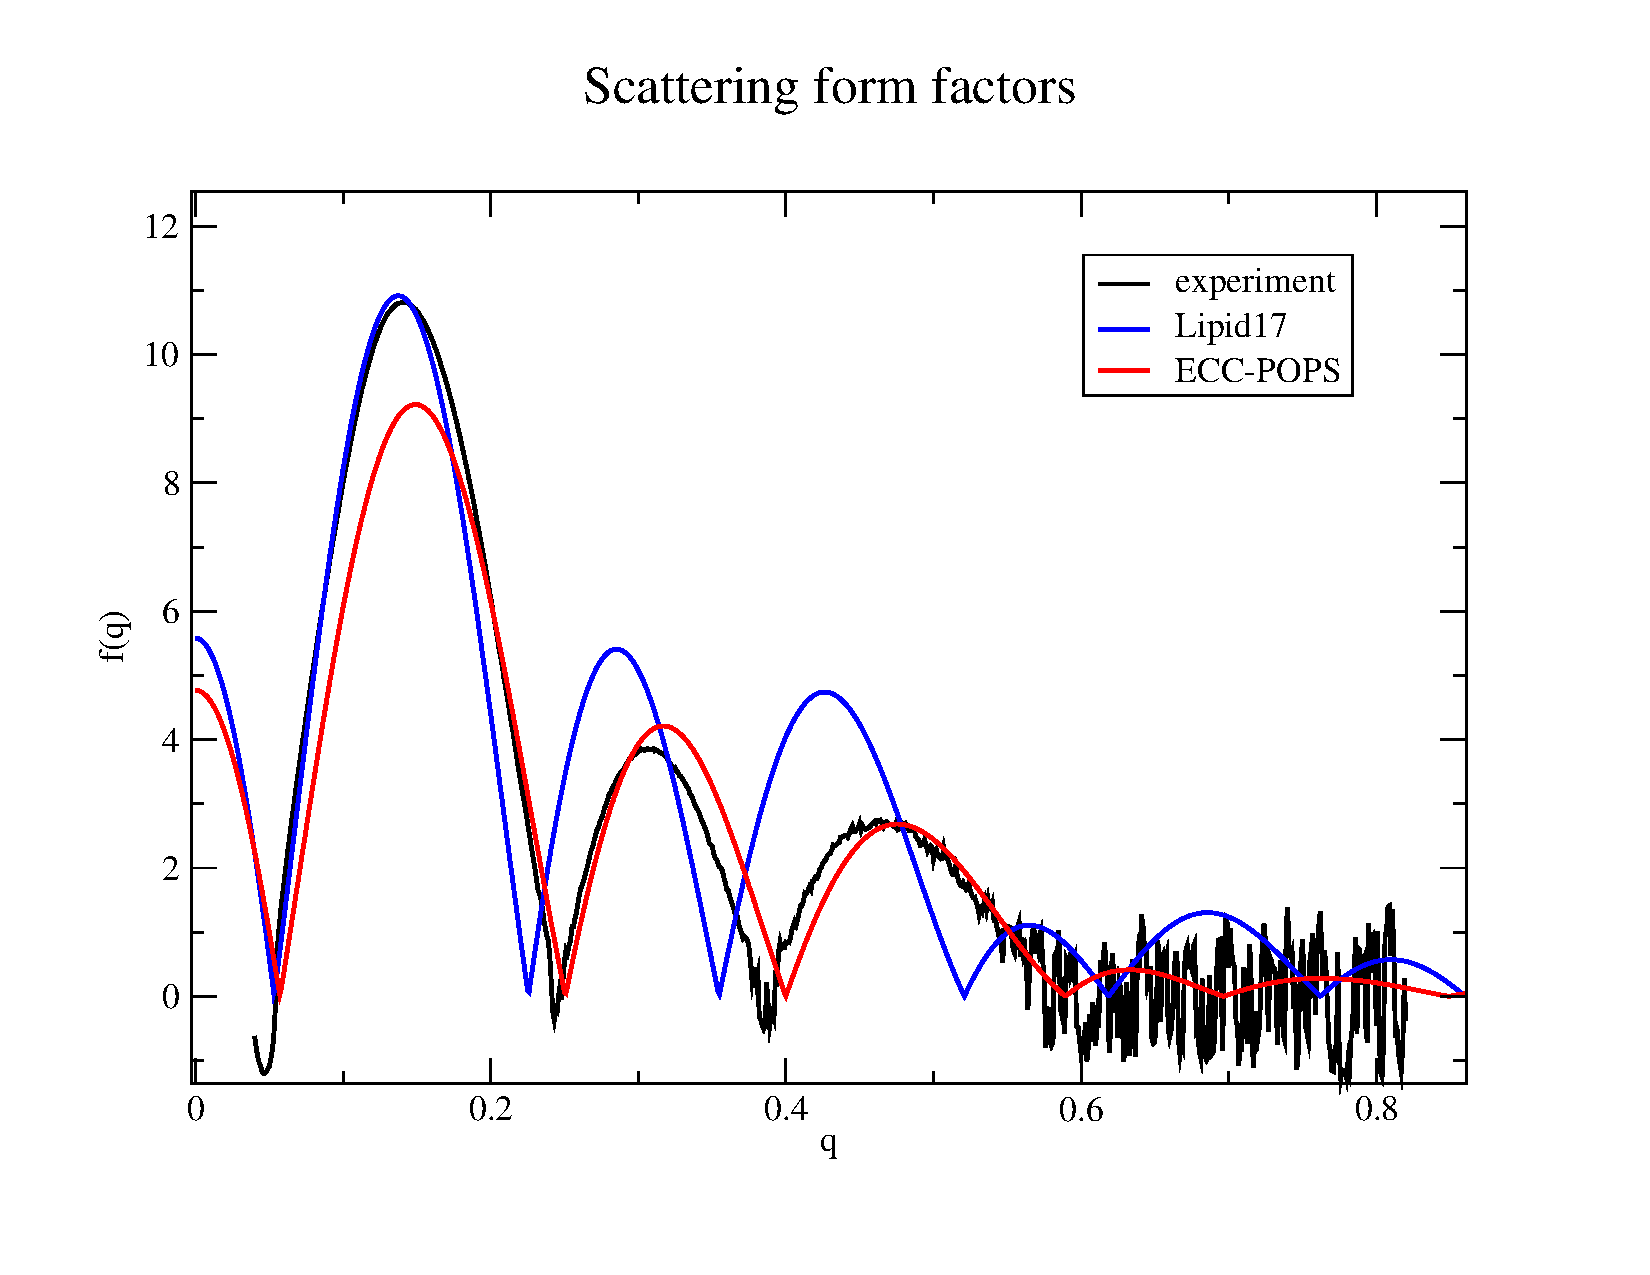
\includegraphics[width=\figwidth]{../img/ecc_pops/form-f_l17-ecc-pops-exp_compar.pdf} 
  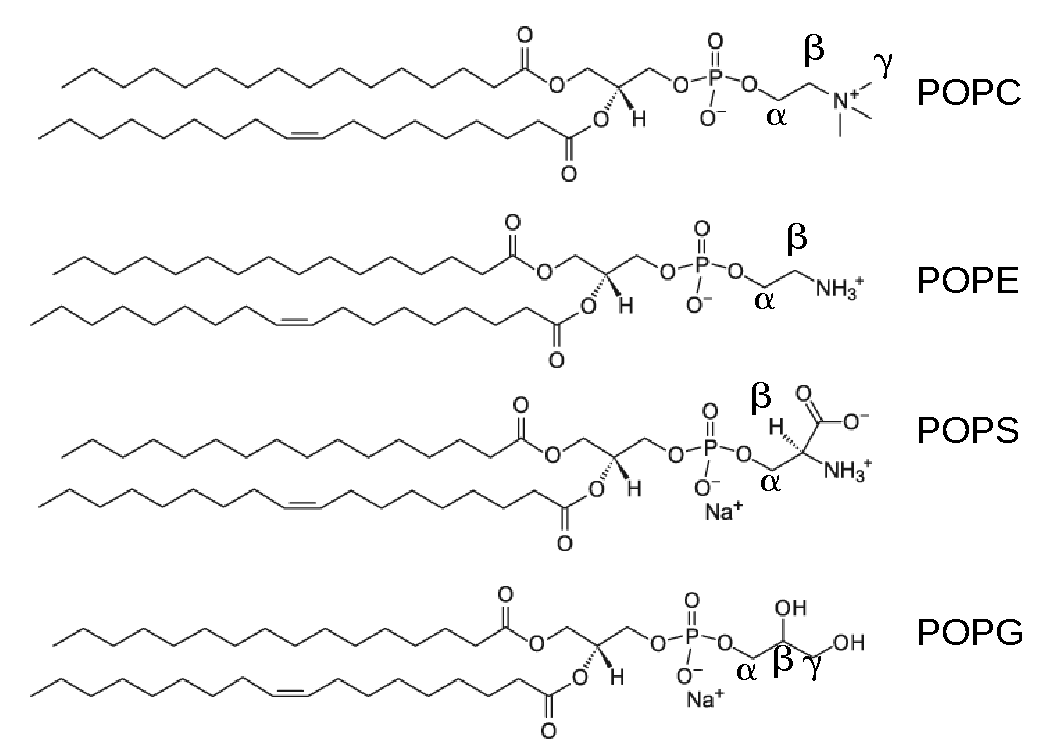
\includegraphics[width=\figwidth]{../img/ecc_pops/lipids_chemfig.pdf} 
  \caption{\label{simVSexpNOions} 
    X-ray scattering form factors from simulations with the Lipid17 \cite{lipid17-future} and 
    the ECC-POPS models compared with experiments~\cite{SDP-CHARMM36_comparison_paper_Samuli-knows} at 298~K. 
    Order parameters of POPS head group, glycerol backbone and acyl chains  
    from simulations with the Lipid17 \cite{lipid17-future} and the ECC-POPS models 
    compared with \emph{experiments at 300~K (check and change)} measured by Tiago Ferriera. 
    Open/closed symbols are used for palmitoyl/oleoyl chains of POPS. 
    The chemical structure of POPS and the labeling of the carbon segments. 
  }  
\end{figure} 
%%%%%%%%%%%%%%%%%%%%%%%%%%%%%%%%%%%%%%%%%%%%%%%%%%%%%%%%%%%%%%
 
\begin{table}[tb!] 
  \caption{Values of the area per lipid (APL) of POPC and POPS bilayers without additional ions. \label{tab:apls} 
  } 
  \begin{tabular}{l|c c} 
    \multicolumn{3}{c}{POPC} \\
    \hline 
    model          & APL (Å$^2$)   & Temperature (K) \\ 
    \hline 
    Lipid14 POPC                    & 65.1$\pm$ 0.6  &  300 \\ 
    Lipid14 POPC \citep{dickson14}  & 65.6$\pm$ 0.5  &  303 \\ 
    \hline 
    ECC-POPC                & 63.2$\pm$ 0.6  &  300       \\ 
    \hline 
    experiment (SDP model) \citep{kucerka11} & 64.3  &  303    \\ 
    \hline 
    \\
    \multicolumn{3}{c}{POPS} \\
    \hline 
    model          & APL (Å$^2$)   & Temperature (K) \\ 
    \hline 
    Lipid17 POPS              & 53.5$\pm$ 0.8  &  298 \\ 
    \hline 
    ECC-POPS                & 60.3$\pm$ 0.6  &  298       \\ 
    \hline 
    experiment (SDP model) \cite{SDP-CHARMM36_comparison_paper_Samuli-knows} & 62.3  &  298    \\ 
    \hline 
  \end{tabular} 
\end{table} 
 
 
First, we present results for bilayers in pure water. 
The ECC-POPC and Lipid14 models both reproduce the experimental X-ray scattering form factors 
of a POPC bilayer with a comparable accuracy (see Fig.~\ref{simVSexpNOions}). 
The area per lipid from the Lipid14 model is by $\approx$1Å larger than the 
experimental value in Table~\ref{tab:apls}, while the value from the ECC-POPC model 
is by $\approx$1Å smaller than the experimental one. 
The values of the area per lipid of the ECC-POPC model vary slightly 
when simulated with different water models (i.e., within the interval of 62.2--66.8 Å, see Table~S2 in SI), 
while still being close to the experimentally reported values. 
We can thus conclude that the ECC-POPC model reproduces the experimental dimensions of the POPC 
lipid bilayer with a comparable accuracy to other state-of-the-art lipid models~\citep{ollila16}. 
 
 
Similarly, the acyl chain order parameters of the ECC-POPC model, as well as those of the Lipid14 model~\citep{dickson14}, agree with the experimental values within the error bars, as presented in Fig.~\ref{simVSexpNOions}. Notably, the experimentally measured forking and small order parameter values of the $C_2$ segment in {\it sn}-2 chain are well reproduced by both models. This feature has been suggested to indicate that the carbonyl of the {\it sn}-2 chain is directed towards the water phase, in contrast to the carbonyl in the {\it sn}-1 chain, which orients more along the bilayer plane~\citep{seelig75,schindler75,gawrisch92}. 
This arrangement, which is not fully reproduced by other available lipid models~\citep{ollila16}, may be a relevant feature for the ion binding details. 
 
The order parameters of the $\alpha$ and $\beta$ carbons in the head group are slightly larger in the ECC-POPC model than in the Lipid14 model, which is apparently related to the P-N vector orienting by about 7$^{\circ}$ more toward the water phase in the former model, see Fig.~\ref{OrderParameterCHANGESsurf}. While both models perform relatively well, considering the available experimental evidence, it is not possible to decide which of the two models provides more realistic head group orientations. The ECC-POPC model gives the $\beta$ carbon order parameter value closer to experiments than the Lipid14 model, while the opposite is true for the $\alpha$ carbon. The accuracy of both models in the glycerol backbone region is comparable to other state-of-the-art lipid model available in literature \citep{botan15}, see Fig.~\ref{simVSexpNOions}. 


 
 
